\subsubsection{Анализ алгоритма идентификации}

Для тестирования алгоритма идентификации использовались различные системы ОДУ 1-ого порядка, найденные в книге \cite{synergetics}. Эволюция систем производилась при помощи \texttt{scipy.integrate.solve\_ivp}, в котором используется явный метод Рунге-Кутты четвертого порядка.

Оценка идентифицированной системы производилась при помощи нескольких метрик. В оценке задачи определения значимых членов важно учитывать и те из них, которые не идентифицировались, и те, которые идентифицировались ложно. Поэтому элементарной метрикой может являться само количество таких членов (метрика ME):

\begin{equation}
ME = (FN,\ FP),
\end{equation}

где $FN$ --- false negative --- число потерянных слагаемых,\par
$FP$ --- false positive --- число ложно определенных слагаемых.

Однако такая метрика может быть не очень удобной, и в качестве метрики, объединяющей эти два числа, выбрана IoU --- intersection over union, также известная как коэффициент Жаккара. Эта метрика показывает какая часть из всех фигурирующих слагаемых (предсказанных и истинных) определена верно:

\begin{equation}
J = \frac{TP}{TP + FP + FN},
\end{equation}

где $TP$ --- true positive --- число верно определенных слагаемых.

После выбора метрик, методы регрессии были протестированы снова, на этот раз применительно к задаче идентификации. Так, выяснилось, что алгоритм Lasso плохо для этого подходит. Если простые системы, например, простейшую систему линейных уравнений~(\ref{eq:linear}), еще получается идентифицировать нормально, как это показано на рисунке~\ref{fig:linear:lasso}. Пример конкретной восстановленной системы изображен на рисунке~\ref{fig:linear:lasso_example}.

\begin{equation}
\normalspacing
\begin{aligned}
\dot{x} &= -0.1 x + 2 y \\
\dot{y} &= -2 x - 0.1 y
\end{aligned}
\label{eq:linear}
\end{equation}

\begin{figure}
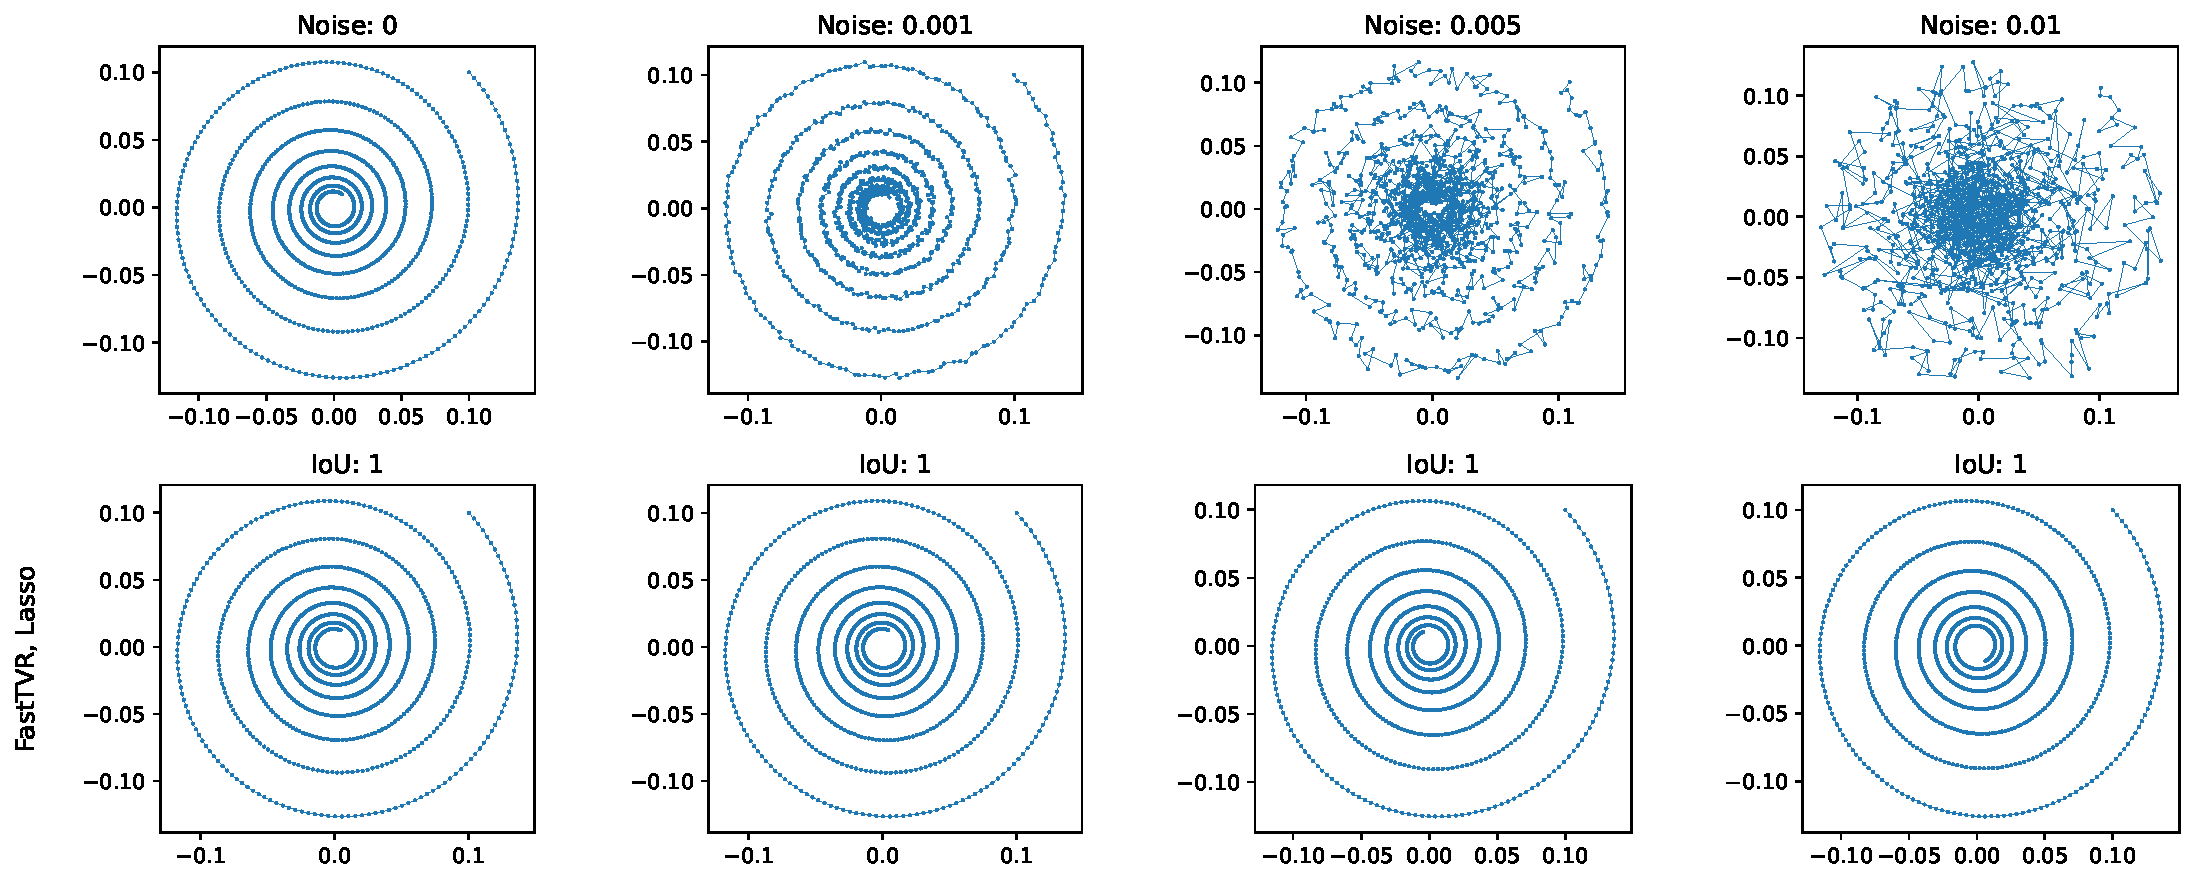
\includegraphics[width=\textwidth]{sindy/linear_lasso}
\caption{Идентификация системы линейных уравнений}
\label{fig:linear:lasso}
\end{figure}

\begin{figure}
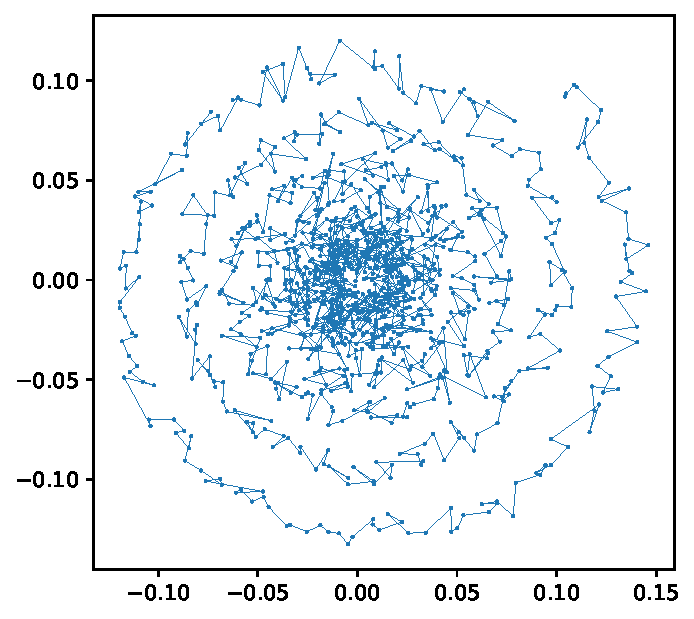
\includegraphics[height=0.28\textheight]{sindy/linear_lasso_orig}\hfill
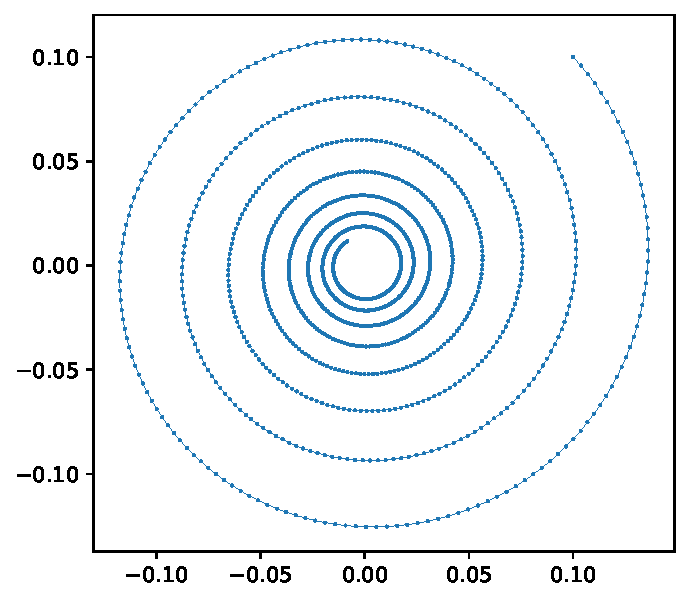
\includegraphics[height=0.28\textheight]{sindy/linear_lasso_res}
\caption{Исходные данные (уровень шума $0.005$) и график восстановленной системы уравнений~(\ref{eq:linear_lasso})}
\label{fig:linear:lasso_example}
\end{figure}

\begin{equation}
\normalspacing
\begin{aligned}
\dot{x} &= -0.115 x + 1.97 y \\
\dot{y} &= -1.94 x - 0.062 y
\end{aligned}
\label{eq:linear_lasso}
\end{equation}

То с более сложными системами возникают проблемы. Это видно на рисунке~\ref{fig:lorenz:lasso}, на котором изображена попытка подбора параметра --- коэффициента регуляризации --- для системы Лоренца. График показывает значения метрики IoU в зависимости от уровня шума и величины параметра, серые пунктирные линии ограничивают область с наибольшим IoU.

\begin{figure}
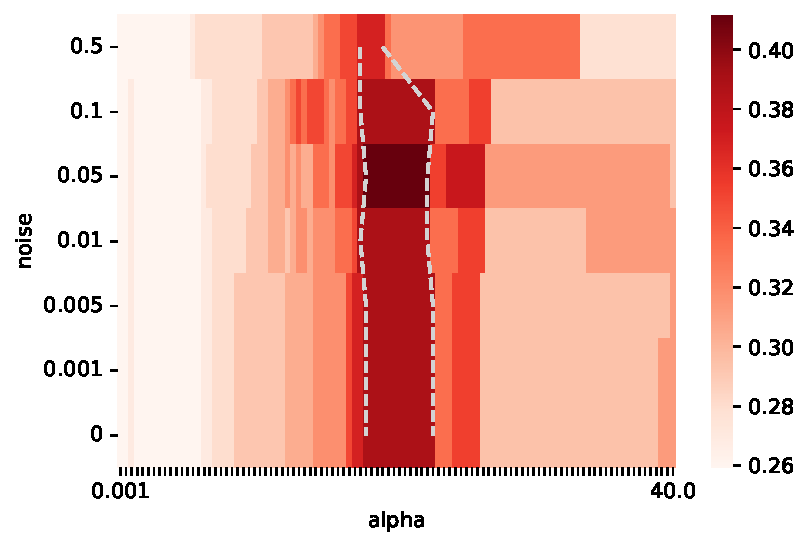
\includegraphics[width=0.9\textwidth]{sindy/lorenz_lasso}
\caption{Подбор параметра $\alpha$ для системы Лоренца}
\label{fig:lorenz:lasso}
\end{figure}

Пример крайне неудачной идентификации показан на рисунке~\ref{fig:lorenz:lasso_example}.

\begin{figure}
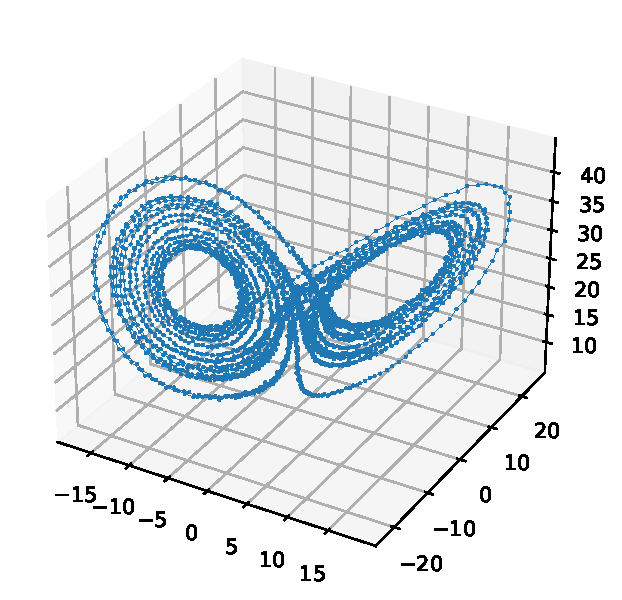
\includegraphics[width=0.49\textwidth]{sindy/lorenz_lasso_orig}\hfill
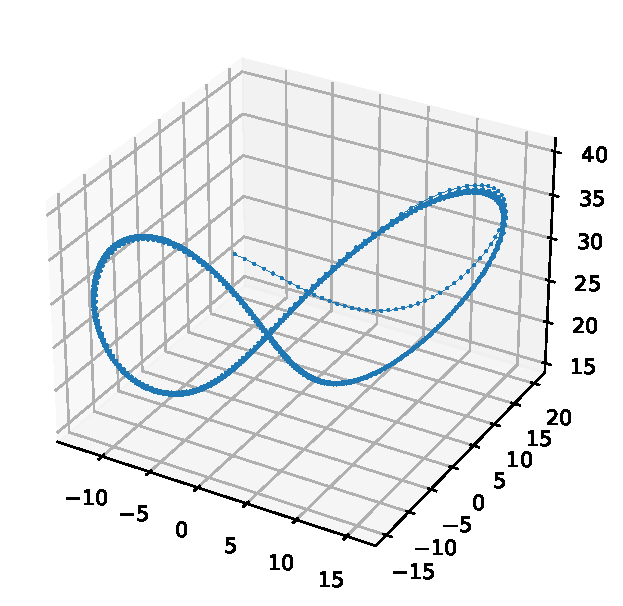
\includegraphics[width=0.49\textwidth]{sindy/lorenz_lasso_res}
\caption{Исходные данные (уровень шума $0.1$) и график восстановленной системы уравнений~(\ref{eq:lorenz_lasso})}
\label{fig:lorenz:lasso_example}
\end{figure}

\begin{equation}
\normalspacing
\begin{aligned}
\dot{x} &= 1.2 y - 0.3 x z + \num{5.1e-4} y^2 + 0.28 y z + 0.0013 z^2 \\
\dot{y} &= 0.47 x + 12 y + 0.0026 x^2 - 0.26 x z - 0.32 y z - 0.004 z^2 \\
\dot{z} &= -0.72 z + 0.57 x^2 + 0.57 x y + \num{9e-5} x z + 0.035 y^2 - 0.088 z^2 \\
\end{aligned}
\label{eq:lorenz_lasso}
\end{equation}

В связи с этим, далее алгоритм Lasso не используется, и в качестве метода регрессии рассматривается только STLSQ.

\paragraph{Система Лоренца}

Систему линейных уравнений решено пропустить из-за ее излишней простоты. Поэтому переходим к аттрактору Лоренца --- решению системы Лоренца (\ref{eq:lorenz}) с начальными значениями $x_0 = 8$, $y_0 = 7$, $z_0 = 27$ и в диапазоне $t \in [0, 20]$. Аттрактор изображен на рисунке~\ref{fig:lorenz}.

\begin{equation}
\normalspacing
\begin{aligned}
\dot{x} &= 10 (y - x) \\
\dot{y} &= x (28 - z) - y \\
\dot{z} &= x y - 8/3 z
\end{aligned}
\label{eq:lorenz}
\end{equation}

\begin{figure}
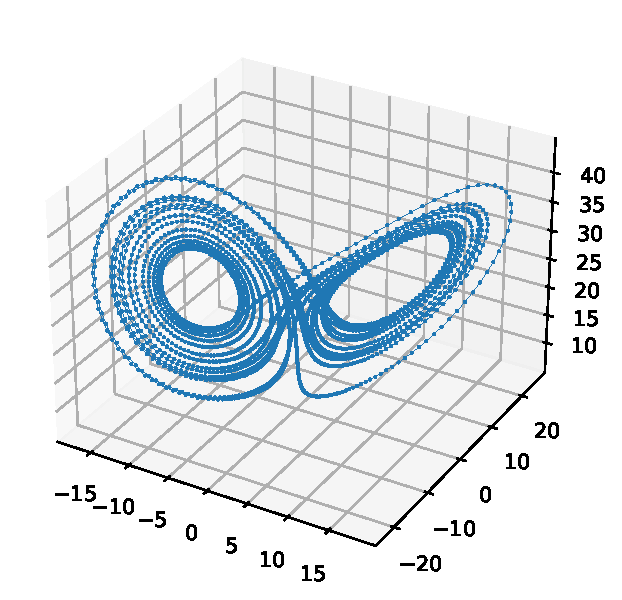
\includegraphics[width=0.5\textwidth]{sindy/lorenz}
\caption{Аттрактор Лоренца}
\label{fig:lorenz}
\end{figure}

Протестируем алгоритм STLSQ. Результаты тестирования изображены на рисунке~\ref{fig:lorenz:stlsq}. Здесь уже наблюдается диапазон значений параметра, при которых достигается приемлемый результат.

\begin{figure}
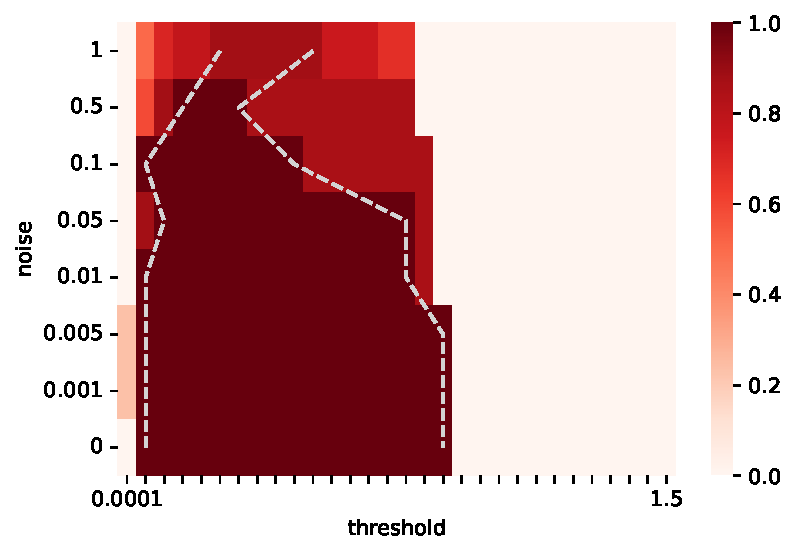
\includegraphics[width=0.49\textwidth]{sindy/lorenz_stlsq_fast_tvr}\hfill
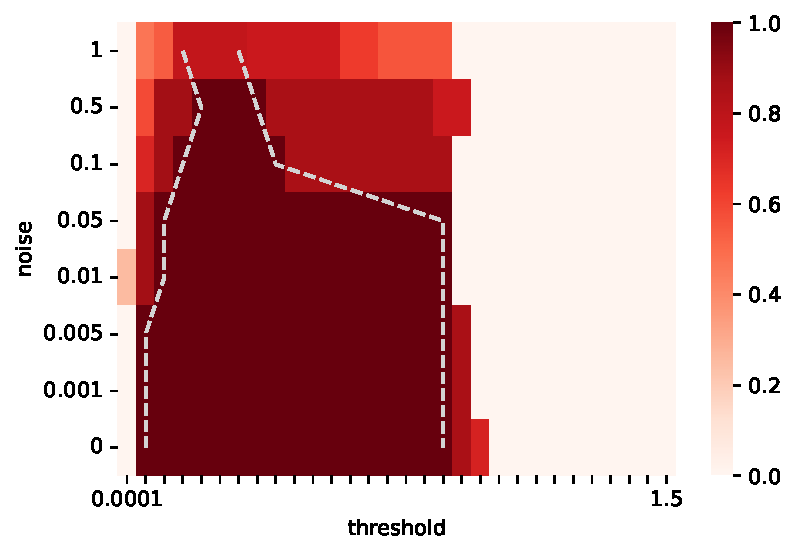
\includegraphics[width=0.49\textwidth]{sindy/lorenz_stlsq_tvr}
\caption{Тестирование алгоритма STLSQ для обоих методов дифференцирования}
\label{fig:lorenz:stlsq}
\end{figure}

Таким образом, имеется возможность подобрать параметры для идентификации системы. На рисунке~\ref{fig:lorenz:test} показаны результаты идентификации вместе со значениями метрики IoU, каждый столбец соответствует одному уровню шума, на первой строке показаны исходные данные.

\begin{figure}
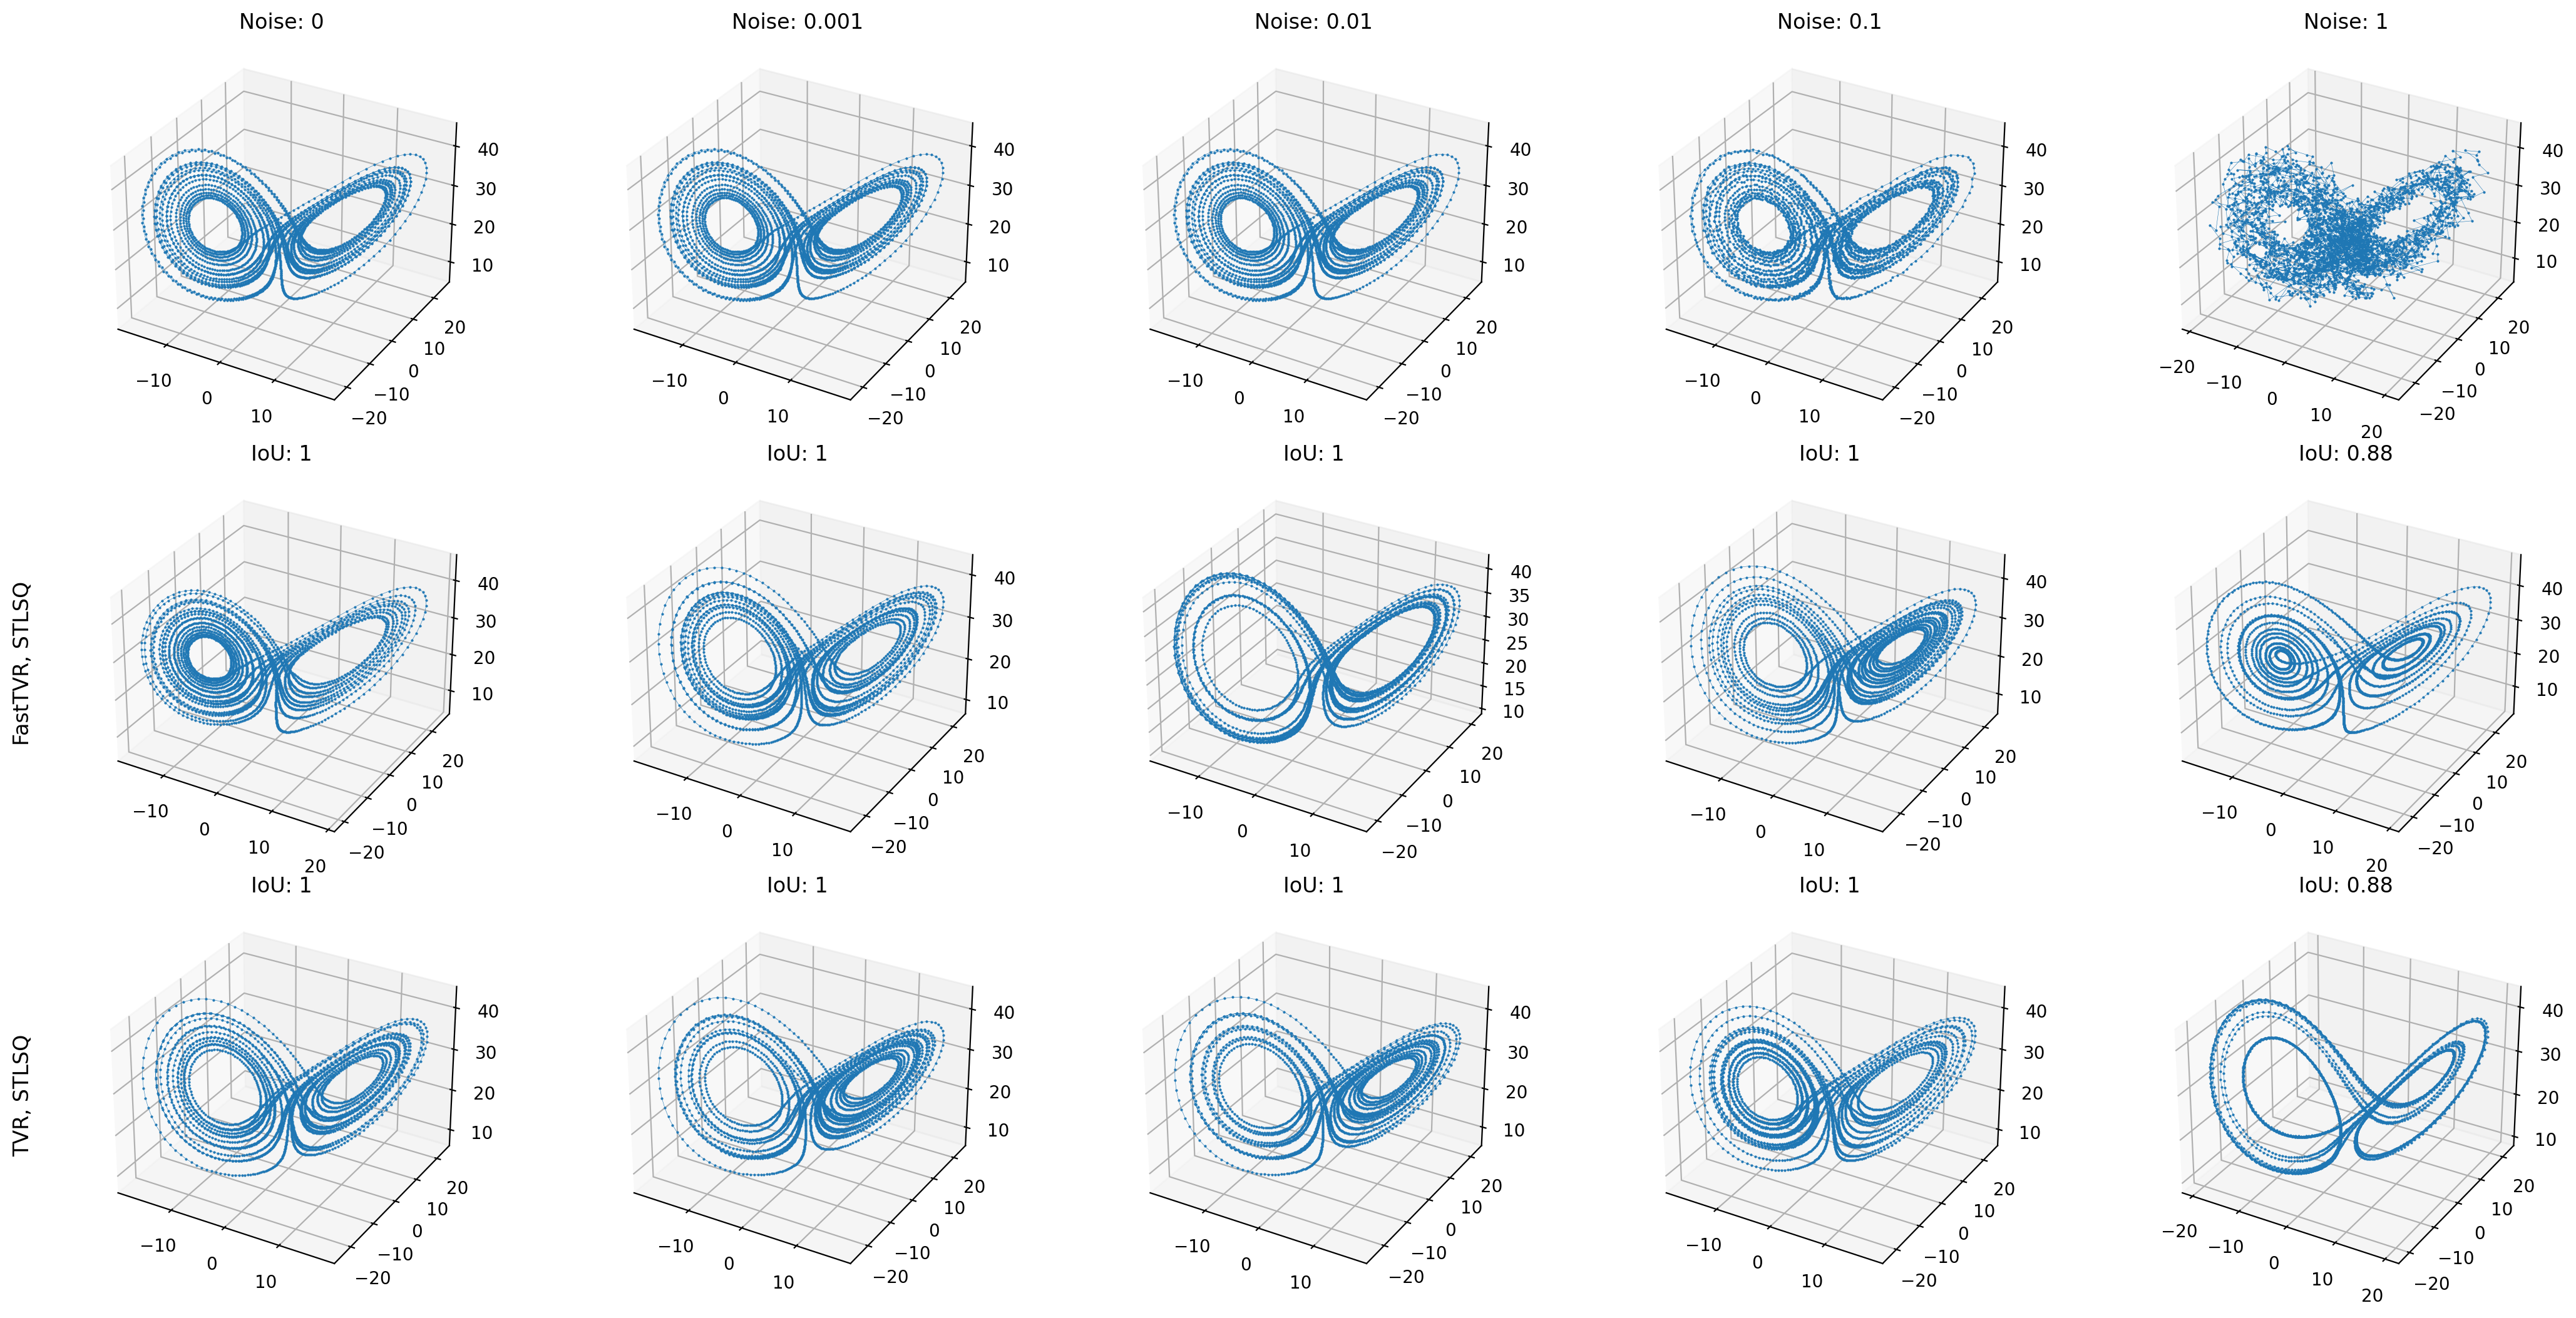
\includegraphics[width=\textwidth]{sindy/lorenz_test}
\caption{Графики восстановленных систем Лоренца}
\label{fig:lorenz:test}
\end{figure}

Можно заметить, что восстановленные системы отличаются от оригинальной. Это связано с тем, что параметры системы восстанавливаются не очень точно. Восстановленные системы уравнений при использовании TVR и уровнях шума $0$, $0.005$, $0.05$, $0.1$, $0.5$ и $1$ имеют следующий вид:

\begin{equation}
\normalspacing
\begin{aligned}
\dot{x} &= -10 x + 10 y                  &\dot{x} &= -9.974 x + 9.979 y \\
\dot{y} &= 27.79 x - 0.917 y - 0.993 x z \qquad &\dot{y} &= 27.78 x - 0.919 y - 0.993 x z \\
\dot{z} &= -2.67 z + 0.999 x y           &\dot{z} &= -2.667 z + 0.999 x y \\
\\
\dot{x} &= -9.97 x + 9.978 y             &\dot{x} &= -9.91 x + 9.928 y \\
\dot{y} &= 27.63 x - 0.861 y - 0.989 x z &\dot{y} &= 27.34 x - 0.833 y - 0.982 x z \\
\dot{z} &= -2.668 z + 0.999 x y          &\dot{z} &= -2.647 z + 0.989 x y \\
\\
\dot{x} &= -9.605 x + 9.683 y        &\dot{x} &= 2.741 - 0.438 x + 4.448 y \\
\dot{y} &= 25.55 x - 0.939 x z       &\dot{y} &= 23.03 x + 0.327 y - 0.877 x z \\
\dot{z} &= 1.2 - 2.658 z + 0.977 x y &\dot{z} &= -2.541 z + 0.955 x y
\end{aligned}
\end{equation}

На рисунке~\ref{fig:lorenz:scores} показаны изменения метрик при использовании TVR: средней ошибки между значениями величин, метрик ME и IoU.

\begin{figure}
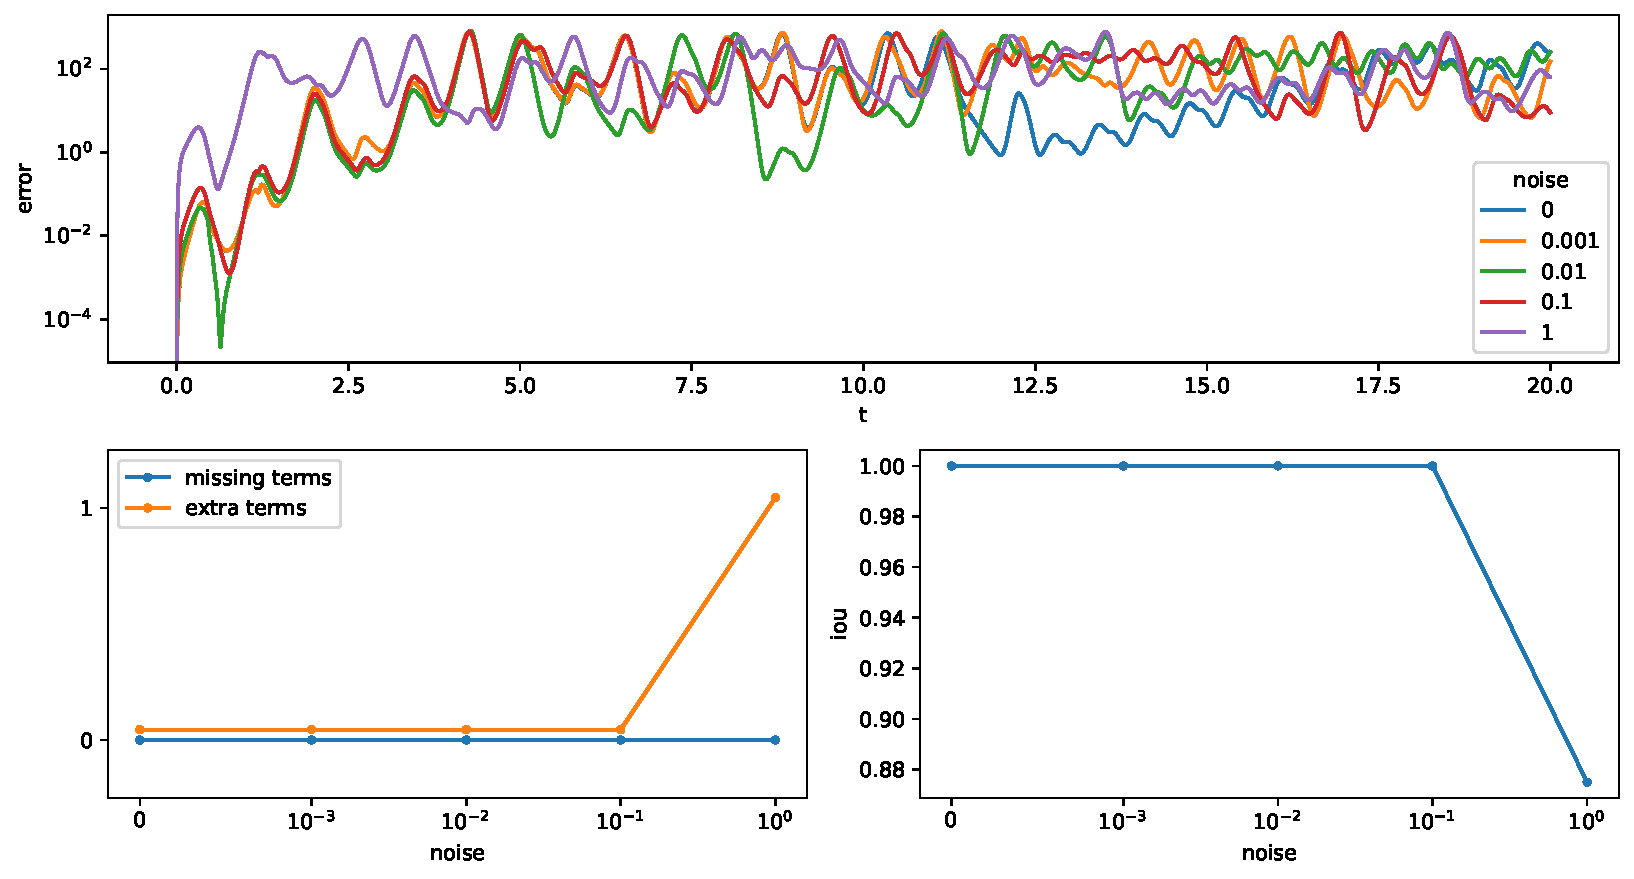
\includegraphics[width=\textwidth]{sindy/lorenz_scores}
\caption{Графики изменения метрик}
\label{fig:lorenz:scores}
\end{figure}

Видно, что, из-за неточных параметров, сравнивать восстановленную систему с исходной напрямую не имеет смысла. Значения средней ошибки получаются большими и примерно одинаковыми для всех случаев. Остальные графики более осмысленные, видно, что число лишних или потерянных слагаемых растет очень незначительно.

\paragraph{Система Мура-Шпигеля}

Система Мура-Шпигеля~(\ref{eq:moore_spiegel}) взята с начальными значениями $x_0 = 0.1$, $y_0 = 0.2$, $z_0 = 0.3$ и в диапазоне $t \in [600, 900]$. Решение системы изображено на рисунке~\ref{fig:moore_spiegel}.

\begin{equation}
\normalspacing
\begin{aligned}
\dot{x} &= y \\
\dot{y} &= z - 0.2 x \\
\dot{z} &= -z / 50 + y (1 - 0.8 x^2)
\end{aligned}
\label{eq:moore_spiegel}
\end{equation}

\begin{figure}
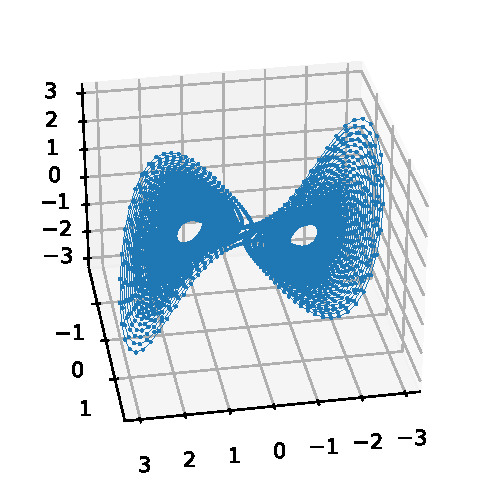
\includegraphics[width=0.5\textwidth]{sindy/moore_spiegel}
\caption{Система Мура-Шпигеля}
\label{fig:moore_spiegel}
\end{figure}

Эту систему было значительно сложнее идентифицировать, как можно видеть из рисунка~\ref{fig:moore_spiegel:test}.

\begin{figure}
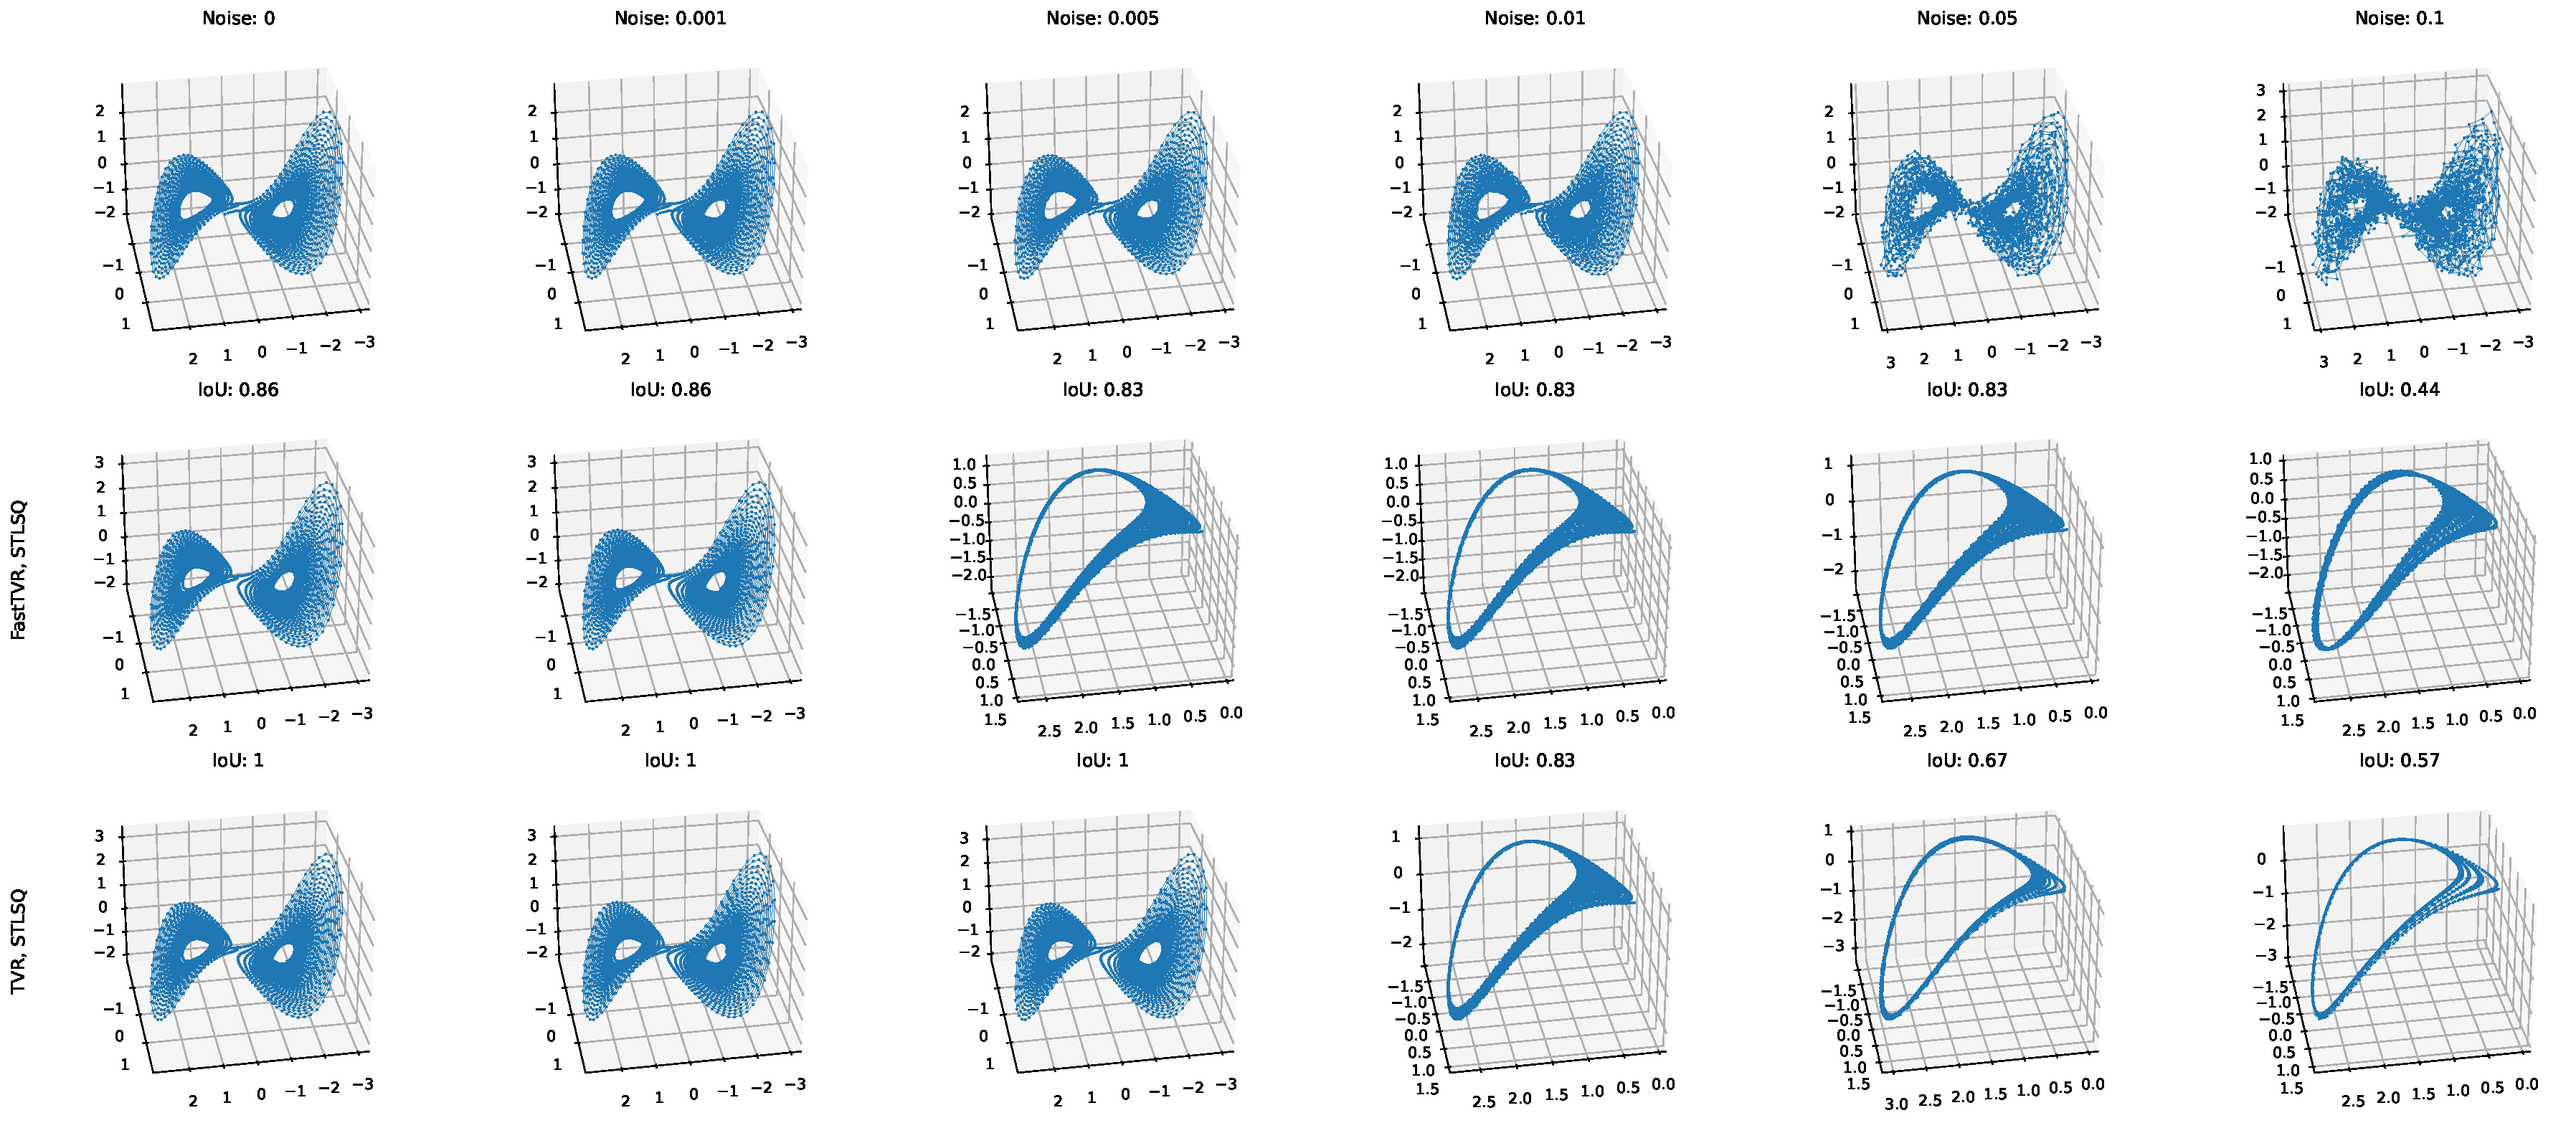
\includegraphics[width=\textwidth]{sindy/moore_spiegel_test}
\caption{Графики восстановленных систем Мура-Шпигеля}
\label{fig:moore_spiegel:test}
\end{figure}

Графики изменения метрик для обоих методов дифференцирования показаны на рисунке~\ref{fig:moore_spiegel:scores}.

\begin{figure}
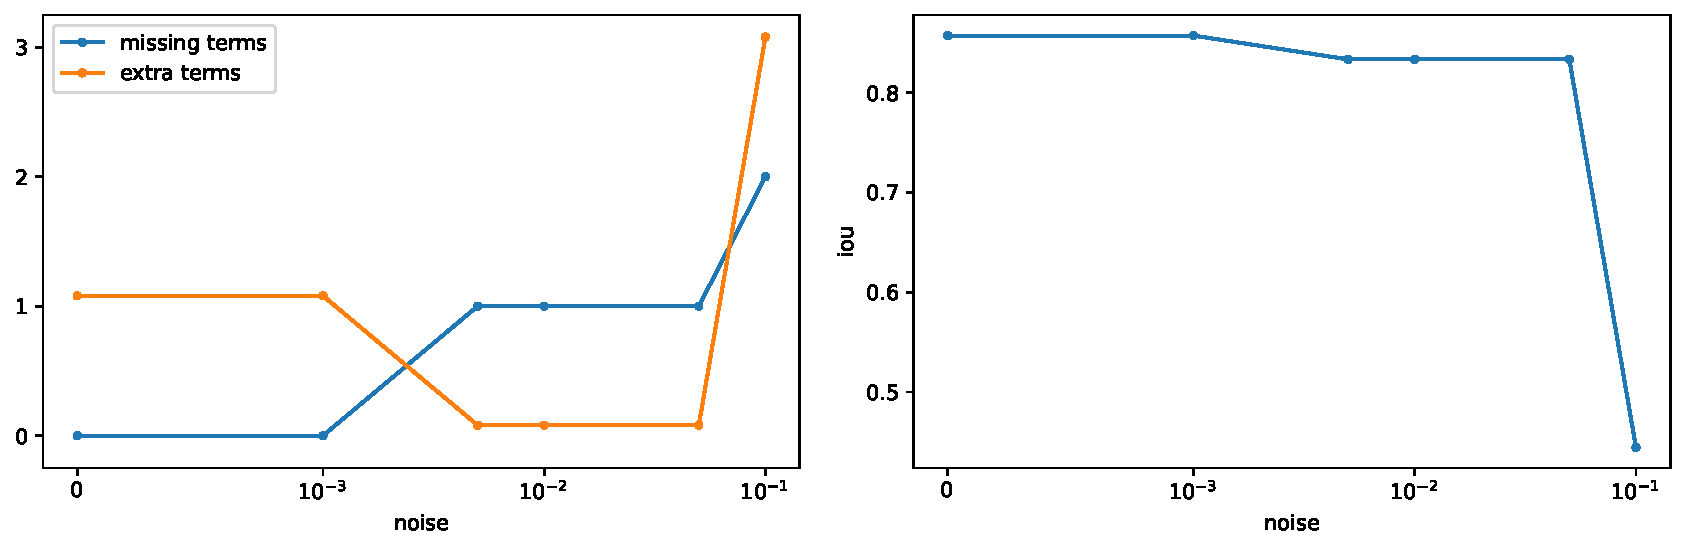
\includegraphics[width=\textwidth]{sindy/moore_spiegel_scores_fast_tvr}
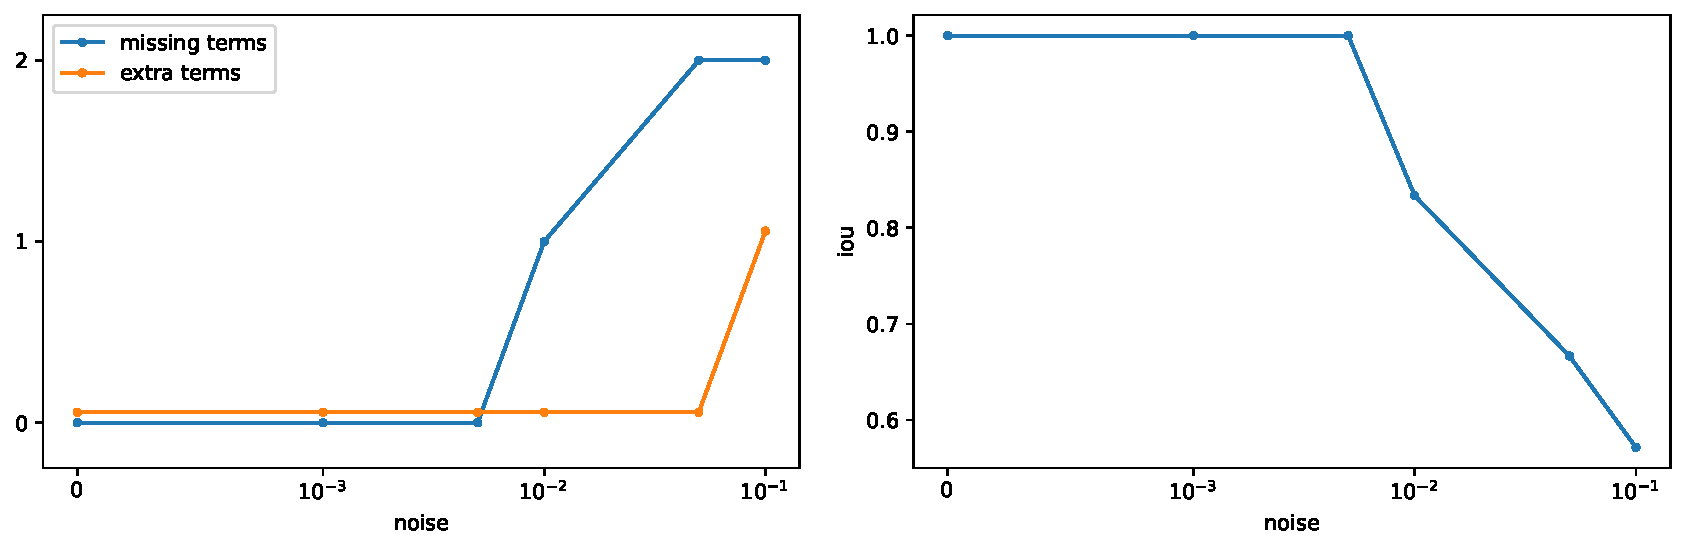
\includegraphics[width=\textwidth]{sindy/moore_spiegel_scores_tvr}
\caption{Графики изменения метрик}
\label{fig:moore_spiegel:scores}
\end{figure}

Ниже приведены восстановленные системы уравнений при использовании TVR, видно, как, начиная с четвертого уровня шума, уравнения теряют слагаемые:

\begin{equation}
\normalspacing
\begin{aligned}
\dot{x} &= 0.977 y                         &\dot{x} &= 0.977 y \\
\dot{y} &= -0.186 x + 0.975 z              &\dot{y} &= -0.186 x + 0.976 z \\
\dot{z} &= 0.992 y - 0.021 z - 0.798 x^2 y \qquad &\dot{z} &= 0.993 y - 0.021 z - 0.799 x^2 y \\
\\
\dot{x} &= 0.984 y                         &\dot{x} &= 0.982 y \\
\dot{y} &= -0.185 x + 0.978 z              &\dot{y} &= -0.187 x + 0.979 z \\
\dot{z} &= 1.006 y - 0.021 z - 0.802 x^2 y &\dot{z} &= 1.046 y - 0.81 x^2 y \\
\\
\dot{x} &= 0.963 y             &\dot{x} &= 0.905 y \\
\dot{y} &= 0.948 z             &\dot{y} &= 0.917 z \\
\dot{z} &= 0.9 y - 0.729 x^2 y &\dot{z} &= 0.757 y - 0.642 x^2 y - 0.167 y z^2
\end{aligned}
\end{equation}